%Template Proposal PA
%Departemen Teknik Elektro dan Informatika
%Sekolah Vokasi UGM

%Dikembangkan oleh Dr. Fahmizal, S.T., M.Sc. dan Tim

%Perangkat lunak yang digunakan untuk mengolah LaTEX pada template ini adalah
%- TeXstudio
%- MiKTex
%- Overleaf (LaTEX editor berbasis daring)

\documentclass[12pt, a4paper, onecolumn, oneside, final]{report}

%Isi identitas proyek akhir disini

\providecommand{\tipe}{Proposal Proyek Akhir}
\providecommand{\permohonan}{Proposal Permohonan Proyek AKhir}
\providecommand{\judul}{(Judul Proyek Akhir yang Diajukan)}

\providecommand{\penulisPertama}{Nama Mahasiswa} 
\providecommand{\nimPertama}{Nomor Induk Mahasiswa}

\providecommand{\prodi}{Teknologi Rekayasa Internet} 
\providecommand{\departemen}{Departemen Teknik Elektro dan Informatika}
\providecommand{\fakultas}{Sekolah Vokasi}
\providecommand{\universitas}{Universitas Gadjah Mada} 

\providecommand{\tglpengesahan}{\today} 
\providecommand{\tglpersetujuan}{\today}
\providecommand{\tglpernyataan}{\today}
\providecommand{\tahun}{\the\year{}} 

\providecommand{\tanggalSeminar}{} 
\providecommand{\waktuSeminar}{} 
\providecommand{\tempatSeminar}{} 

\providecommand{\dosenPembimbingI}{Nama Dosen Pembimbing I} 
\providecommand{\dosenPembimbingII}{Nama Dosen Pembimbing II} 
\providecommand{\ketuaProgramStudi}{Nama Ketua Program Studi} 

\providecommand{\nipDosenPembimbingI}{XXXXXXXXXXXXXXXX} 
\providecommand{\nipDosenPembimbingII}{XXXXXXXXXXXXXXXX} 
\providecommand{\nipKetuaProgramStudi}{XXXXXXXXXXXXXXXX} 

\providecommand{\katakunci}{kata kunci 1, kata kunci 2, kata kunci 3}

% Mengatur bahasa & encoding latex
\usepackage[indonesian]{babel}
\usepackage[utf8]{inputenc}

% Untuk pengaturan spacing
\usepackage{setspace}
\onehalfspacing

% Untuk mengatur level section 
\setcounter{secnumdepth}{6}

% Digunakan untuk memasukan gambar ke laporan. 
\usepackage{graphicx}
\graphicspath{{gambar/}}
\usepackage{float}
\usepackage[hang,centerlast, nooneline ,small,md]{subfigure}
\usepackage[subfigure]{tocloft}

% Untuk mengatur spacing antara paragraf
\usepackage{parskip}

% Membuat indent
\usepackage{indentfirst}
\setlength\parindent{1cm}

% Untuk mengkustomisasi margin
\usepackage{scrextend}

% Untuk mengatur header dan footer
\usepackage{fancyhdr}

% Membuat seluruh tulisan menjadi Times New Roman. 
% \usepackage{pslatex}

% Merubah numbering chapter dan section untuk judul setiap bab menggunakan romawi dan judul anak bab menggunakan arabic
\renewcommand{\thesection}{\arabic{chapter}.\arabic{section}\hspace{0.05cm}}
\renewcommand{\thesubsection}{\arabic{chapter}.\arabic{section}.\arabic{subsection}\hspace{-0.25cm}}
\renewcommand{\thesubsubsection}{\Alph{subsubsection}.\hspace{-0,25cm}}

% Mengatur identasi judul section dan subsection
%\titleformat{\section}[block]{\bfseries}{\thesection.}{1em}{}
%\titleformat{\subsection}[block]{\hspace{2em}}{\thesubsection}{1em}{}

% Merubah huruf kapital pada judul daftar isi, daftar gambar, dan daftar table
\usepackage{tocloft}
\renewcommand{\cfttoctitlefont}{\hfil\large\bfseries\MakeUppercase}
\renewcommand{\cftloftitlefont}{\hfil\large\bfseries\MakeUppercase}
\renewcommand{\cftlottitlefont}{\hfil\large\bfseries\MakeUppercase}

\renewcommand\cftchappresnum{BAB }
\renewcommand\cftchapaftersnum{}
\newlength\mylen
\settowidth\mylen{\bfseries BAB 1 :\ } % if more than 9 chapters, use "Chapter 10"
\cftsetindents{chap}{0pt}{\mylen}

% Untuk merupakan format penulisan BAB
\usepackage{titlesec}
\titleformat{\chapter}
{\doublespacing\fontsize{14pt}{16pt}\bfseries}
{\MakeUppercase{\chaptertitlename\ \Roman{chapter}}\filcenter}
{0.15cm}{\centering\uppercase}

% Mengatur spacing section
\titleformat{\section}
  {\fontsize{12}{14}\selectfont\bfseries}{\thesection}{1em}{}
\titleformat{\subsection}
  {\fontsize{12}{14}\selectfont\bfseries}{\thesubsection}{1em}{}
\titleformat{\subsubsection}
  {\fontsize{12}{14}\selectfont\bfseries}{\thesubsubsection}{1em}{}

\titlespacing*{\section}{0pt}{10pt}{0cm}
\titlespacing*{\subsection}{0pt}{10pt}{0cm}
\titlespacing*{\subsubsection}{0pt}{10pt}{0cm}

% Digunakan untuk mengatur caption dalam dokumen.
\usepackage[font=footnotesize,format=plain,labelfont=bf,up,textfont=up]{caption}

% Untuk menghapus titik dua (colon)
\captionsetup[figure]{labelsep=space}
\captionsetup[table]{labelsep=space}

% Mengatur nomor caption gambar
\renewcommand{\thefigure}{\arabic{chapter}.\arabic{figure}}

% Mengatur nomor caption table
\renewcommand{\thetable}{\arabic{chapter}.\arabic{table}}

% Mengatur Hyphenation pada latex
\tolerance=1
\emergencystretch=\maxdimen
\hyphenpenalty=10000
\hbadness=10000

% Untuk mengatur setting indent
\setlength\parindent{1cm}

% Untuk memasukkan table
\usepackage{tabularx}
\usepackage{multirow}

% Untuk mengatur width
\usepackage{changepage}

% Menggatur setting halaman 
\usepackage{geometry}
\geometry{
    left=3cm,            % <-- you want to adjust this
    top=3cm,
    right=2.5cm,
    bottom=3cm,
}

% Teks testing
\usepackage{blindtext}
\usepackage{lipsum}

% Untuk formatting quote pada halaman motto
\usepackage{epigraph}

% Untuk mengatur wrap picture
\usepackage{wrapfig}

% Untuk notasi matematika
\usepackage{amsmath}
\usepackage{stmaryrd}
\usepackage{mathtools}



% untuk mengatur label nomor pada rumus
\renewcommand{\theequation}{\arabic{chapter}.\arabic{equation}}

% Untuk mengatur spacing daftar gambar
\newcommand*{\noaddvspace}{\renewcommand*{\addvspace}[1]{}}
\addtocontents{lof}{\protect\noaddvspace}

%Menambahkan sumber gambar
\usepackage{url}
\newcommand*{\putsource}[1]{%
	\textbf{\small{Sumber: }} \small{\url{#1}}
}

%untuk mengatur package include table in excel
% \usepackage{pgfplotstable}

% untuk mengatur landscape page
\usepackage{rotating}

%untuk mengubah page menjadi landscape
\usepackage{pdflscape}

% untuk list
\usepackage{enumitem}
\newenvironment{packed_enum}{
    \begin{enumerate}[leftmargin=1.5\parindent]
        \setlength{\itemsep}{0pt}
        \setlength{\parskip}{0pt}
        \setlength{\parsep}{0pt}
        }{\end{enumerate}}

\newenvironment{packed_item}{
    \begin{itemize}[leftmargin=1.5\parindent]
        \setlength{\itemsep}{0pt}
        \setlength{\parskip}{0pt}
        \setlength{\parsep}{0pt}
        }{\end{itemize}}

%paket untuk bibTex
\usepackage{cite}
\bibliographystyle{IEEEtran}
% \bibliographystyle{apalike}

%paket untuk mengembed kode dalam LaTeX
\usepackage{listings}
\lstset{
    basicstyle=\small,
    %basicstyle=\ttfamily,
    columns=fullflexible,
    frame=single,
}

%paket untuk tabel
\usepackage{longtable}
\usepackage[table,xcdraw]{xcolor}
\usepackage{tabularx}
\usepackage{multirow}

%paket untuk url
% \usepackage{hyperref}
\usepackage[hidelinks]{hyperref} %remove red boxes

% styling python
\usepackage{color}
\usepackage{listings}    
\usepackage{courier}

\definecolor{mygreen}{rgb}{0,0.6,0}
\definecolor{mygray}{rgb}{0.5,0.5,0.5}
\definecolor{mymauve}{rgb}{0.58,0,0.82}

\lstset{ %
  backgroundcolor=\color{white},   % choose the background color
  basicstyle=\footnotesize,        % size of fonts used for the code
  breaklines=true,                 % automatic line breaking only at whitespace
  captionpos=b,                    % sets the caption-position to bottom
  commentstyle=\color{mygreen},    % comment style
  escapeinside={\%*}{*)},          % if you want to add LaTeX within your code
  keywordstyle=\color{blue},       % keyword style
  stringstyle=\color{mymauve},     % string literal style
}

%styling Processing
\usepackage{verbatim}

%Define Colors
\definecolor{black}{RGB}{0,0,0}
\definecolor{gray}{RGB}{102,102,102}		%#666666
\definecolor{function}{RGB}{0,102,153}		%#006699 lightblue
\definecolor{lightgreen}{RGB}{102,153,0}	%#669900
\definecolor{bluegreen}{RGB}{51,153,126}	%#33997e
\definecolor{magenta}{RGB}{217,74,122}	%#d94a7a
\definecolor{orange}{RGB}{226,102,26}		%#e2661a
\definecolor{purple}{RGB}{125,71,147}		%#7d4793
\definecolor{green}{RGB}{113,138,98}		%#718a62

\lstdefinelanguage{Processing}{
	%keyword1&2&6
	morekeywords = [3]{abstract, break, class, continue, default, enum, extends, false, final, finally, implements, import, instanceof, interface, native, new, null, package, private, protected, public, static, strictfp, throws, transient, true, void, volatile, length, assert, case, return, super, this, throw},
	%keyword3
	morekeywords = [4]{catch, do, for, if, else, switch, synchronized, while, try},
	%keyword4
	morekeywords = [5]{width, height, pixelHeight, displayHeight, displayWidth, focused, frameCount, frameRate, key, keyCode, keyPressed, mouseButton, mousePressed, mouseX, mouseY, pixels, pixelWidth, pmouseX, pmouseY},
	%keyword5
	morekeywords = [6]{Array, ArrayList, Boolean, Byte, BufferedReader, Character, Class, Double, Float, Integer, HashMap, PrintWriter, String, StringBuffer, StringBuilder, Thread, boolean, byte, char, color, double, float, int, long, short, FloatDict, FloatList, IntDict, IntList, JSONArray, JSONObject, PFont, PGraphics, PImage, PShader, PShape, PVector, StringDict, StringList, Table, TableRow, XML},
	%literal2
	morekeywords = [7]{ADD, ALIGN_CENTER, ALIGN_LEFT, ALIGN_RIGHT, ALPHA, ALPHA_MASK, ALT, AMBIENT, ARC, ARROW, ARGB, BACKSPACE, BASELINE, BEVEL, BLEND, BLUE_MASK, BLUR, BOTTOM, BOX, BURN, CENTER, CHATTER, CHORD, CLAMP, CLICK, CLOSE, CMYK, CODED, COMPLAINT, COMPOSITE, COMPONENT, CONCAVE_POLYGON, CONTROL, CONVEX_POLYGON, CORNER, CORNERS, CROSS, CUSTOM, DARKEST, DEGREES, DEG_TO_RAD, DELETE, DIAMETER, DIFFERENCE, DIFFUSE, DILATE, DIRECTIONAL, DISABLE_ACCURATE_2D, DISABLE_DEPTH_MASK, DISABLE_DEPTH_SORT, DISABLE_DEPTH_TEST, DISABLE_NATIVE_FONTS, DISABLE_OPENGL_ERRORS, DISABLE_PURE_STROKE, DISABLE_TEXTURE_MIPMAPS, DISABLE_TRANSFORM_CACHE, DISABLE_STROKE_PERSPECTIVE, DISABLED, DODGE, DOWN, DRAG, DXF, ELLIPSE, ENABLE_ACCURATE_2D, ENABLE_DEPTH_MASK, ENABLE_DEPTH_SORT, ENABLE_DEPTH_TEST, ENABLE_NATIVE_FONTS, ENABLE_OPENGL_ERRORS, ENABLE_PURE_STROKE, ENABLE_TEXTURE_MIPMAPS, ENABLE_TRANSFORM_CACHE, ENABLE_STROKE_PERSPECTIVE, ENTER, EPSILON, ERODE, ESC, EXCLUSION, EXIT, FX2D, GIF, GRAY, GREEN_MASK, GROUP, HALF, HALF_PI, HAND, HARD_LIGHT, HINT_COUNT, HSB, IMAGE, INVERT, JAVA2D, JPEG, LEFT, LIGHTEST, LINE, LINES, LINUX, MACOSX, MAX_FLOAT, MAX_INT, MIN_FOAT, MIN_INT, MITER, MODEL, MOVE, MULTIPLY, NORMAL, NORMALIZED, NO_DEPTH_TEST, NTSC, ONE, OPAQUE, OPEN, ORTHOGRAPHIC, OVERLAY, PAL, PDF, P2D, P3D, PERSPECTIVE, PI, PIE, PIXEL_CENTER, POINT, POINTS, POSTERIZE, PRESS, PROBLEM, PROJECT, QUAD, QUAD_STRIP, QUADS, QUARTER_PI, RAD_TO_DEG, RADIUS, RADIANS, RECT, RED_MASK, RELEASE, REPEAT, REPLACE, RETURN, RGB, RIGHT, ROUND, SCREEN, SECAM, SHAPE, SHIFT, SPAN, SPECULAR, SPHERE, SOFT_LIGHT, SQUARE, SUBTRACT, SVG, SVIDEO, TAB, TARGA, TAU, TEXT, TFF, THIRD_PI, THRESHOLD, TIFF, TOP, TRIANGLE, TRIANGLE_FAN, TRIANGLES, TRIANGLE_STRIP, TUNER, TWO, TWO_PI, UP, WAIT, WHITESPACE},
	%function1
	morekeywords = [8]{start, stop, breakShape, createPath, loadMatrix, parseBoolean, parseByte, parseChar, parseFloat, parseInt, saveFile, savePath, sketchFile, sketchPath, abs, acos, alpha, ambient, ambientLight, append, applyMatrix, arc, arrayCopy, asin, atan, atan2, background, beginCamera, beginContour, beginRaw, beginRecord, beginShape, bezier, bezierDetail, bezierPoint, bezierTangent, bezierVertex, binary, blend, blendColor, blendMode, blue, box, brightness, camera, ceil, circle, clear, clip, color, colorMode, concat, constrain, copy, cos, createFont, createGraphics, createImage, createInput, createOutput, createReader, createShape, createWriter, cursor, curve, curveDetail, curvePoint, curveTangent, curveTightness, curveVertex, day, degrees, delay, directionalLight, displayDensity, dist, ellipse, ellipseMode, emissive, endCamera, endContour, endRaw, endRecord, endShape, exit, exp, expand, fill, filter, floor, frustum, fullScreen, get, green, hex, hint, hour, hue, image, imageMode, join, launch, lerp, lerpColor, lightFalloff, lights, lightSpecular, line, loadBytes, loadFont, loadImage, loadJSONArray, loadJSONObject, loadPixels, loadShader, loadShape, loadStrings, loadTable, loadXML, log, loop, mag, map, match, matchAll, max, millis, min, minute, modelX, modelY, modelZ, month, nf, nfc, nfp, nfs, noClip, noCursor, noFill, noise, noiseDetail, noiseSeed, noLights, noLoop, norm, normal, noSmooth, noStroke, noTint, ortho, parseJSONArray, parseJSONObject, parseXML, perspective, list, pixelDensity, point, pointLight, popMatrix, popStyle, pow, print, printArray, printCamera, println, printMatrix, printProjection, pushMatrix, pushStyle, quad, quadraticVertex, radians, random, randomGaussian, randomSeed, rect, rectMode, red, redraw, requestImage, resetMatrix, resetShader, reverse, rotate, rotateX, rotateY, rotateZ, round, saturation, save, saveBytes, saveFrame, saveJSONArray, saveJSONObject, saveStream, saveStrings, saveTable, saveXML, scale, screenX, screenY, screenZ, second, selectFolder, selectInput, selectOutput, set, shader, shape, shapeMode, shearX, shearY, shininess, shorten, sin, size, smooth, sort, specular, sphere, sphereDetail, splice, split, splitTokens, spotLight, sq, sqrt, square, stroke, strokeCap, strokeJoin, strokeWeight, subset, tan, text, textAlign, textAscent, textDescent, textFont, textLeading, textMode, textSize, texture, textureMode, textureWrap, textWidth, thread, tint, translate, triangle, trim, unbinary, unhex, updatePixels, vertex, year},
	%function2
	morekeywords = [9]{cache, readLine, close, flush, print, println, charAt, equals, indexOf, substring, toLowerCase, toUpperCase, getDouble, getLong, getColumnTitles, getColumnTypes, getColumnType, setDouble, setLong, add, clear, div, get, hasKey, keyArray, keys, mult, remove, set, size, sortKeys, sortKeysReverse, sortValues, sortValuesReverse, sub, valueArray, values, append, array, hasValue, max, min, mult, remove, reverse, shuffle, sort, sortReverse, increment, getBoolean, getFloat, getInt, getIntArray, getJSONArray, getJSONObject, getString, getStringArray, isNull, setBoolean, setFloat, setInt, setJSONArray, setJSONObject, setString, beginDraw, endDraw, blend, copy, filter, loadPixels, mask, resize, save, updatePixels, addChild, beginContour, beginShape, disableStyle, enableStyle, endContour, endShape, getChild, getChildCount, getVertex, getVertexCount, isVisible, resetMatrix, rotate, rotateX, rotateY, rotateZ, scale, setFill, setStroke, setVertex, setVisible, translate, angleBetween, cross, dist, dot, fromAngle, heading, lerp, limit, mag, magSq, normalize, random2D, random3D, setMag, lower, upper, addColumn, addRow, clearRows, findRow, findRows, getColumnCount, getRow, getRowCount, getStringColumn, matchRow, matchRows, removeColumn, removeRow, removeTokens, rows, trim, getColumnTitle, format, getAttributeCount, getChildren, getContent, getName, getParent, hasAttribute, hasChildren, listAttributes, listChildren, removeChild, setContent, setName, toString},
	%function4
	morekeywords = [10]{draw, keyReleased, keyTyped, mouseClicked, mouseDragged, mouseMoved, mouseReleased, mouseWheel, settings, setup},
	keywordstyle = [3]\color{bluegreen},
	keywordstyle = [4]\color{lightgreen},
	keywordstyle = [5]\color{magenta},
	keywordstyle = [6]\color{orange},
	keywordstyle = [7]\color{green},
	keywordstyle = [8]\color{function},
	keywordstyle = [9]\color{function},
	keywordstyle = [10]\color{function}\bfseries,
	sensitive = true,
	morecomment = [l][\color{gray}]{//},
	morecomment = [s][\color{gray}]{/*}{*/},
	morecomment = [s][\color{gray}]{/**}{*/},
	morestring = [b][\color{purple}]",
	morestring = [b][\color{purple}]'
}
\renewcommand{\ttdefault}{pcr}
\lstset{
	language={Processing},
	basicstyle={\small\ttfamily},
	identifierstyle={\small},
	commentstyle={\small\itshape},
	keywordstyle={\small},
	ndkeywordstyle={\small},
	stringstyle={\small\ttfamily},
	frame={tb},
	breaklines=true,
	columns=[l]{fullflexible},
	numbers=left,
	xrightmargin=0em,
	xleftmargin=3em,
	numberstyle={\scriptsize},
	stepnumber=1,
	numbersep=1em,
	lineskip=-0.5ex,
}

%listing style

\definecolor{codegreen}{rgb}{0,0.6,0}
\definecolor{codegray}{rgb}{0.5,0.5,0.5}
\definecolor{codepurple}{rgb}{0.58,0,0.82}
\definecolor{backcolour}{rgb}{0.95,0.95,0.92}

\lstdefinestyle{custom}{
	frame = single,
	backgroundcolor=\color{backcolour},   
	commentstyle=\color{codegreen},
	keywordstyle=\color{magenta},
	numberstyle=\tiny\color{codegray},
	stringstyle=\color{codepurple},
	basicstyle=\ttfamily\footnotesize,
	breakatwhitespace=false,         
	breaklines=true,                 
	captionpos=b,                    
	keepspaces=true,                 
	numbers=left,                    
	numbersep=6pt,                  
	showspaces=false,                
	showstringspaces=false,
	showtabs=false,                  
	tabsize=2
}

\lstset{style=custom}

%memasukan PDF
\usepackage{pdfpages}

\input{chapters/database.hyphenate}

\begin{document}
\begin{titlepage}
    \begin{center}

        \begin{doublespace}
            \textbf{\MakeUppercase{\large{\tipe}}}\\[0.5cm]
            \textbf{\MakeUppercase{\normalsize{\judul}}}\\[4cm]
        \end{doublespace} 
        
        \includegraphics[width=0.35\linewidth]{gambar/logo-ugm.png}\\[2cm]

        \textbf{\large {Oleh:}} \\
        
        \textbf{\normalsize \MakeUppercase{\underline{\penulisPertama}}} \\
        \textbf{\normalsize \MakeUppercase{{\nimPertama}}} \\[2cm]

        \textbf{\normalsize \MakeUppercase{Program Studi Sarjana Terapan}}\\
        \textbf{\normalsize \MakeUppercase{\prodi}}\\
        \textbf{\normalsize \MakeUppercase{\departemen}}\\
        \textbf{\normalsize \MakeUppercase{\fakultas}}\\
        \textbf{\normalsize \MakeUppercase{\universitas}}\\
        \textbf{\normalsize \the\year{}}\\
    \end{center}
\end{titlepage}

\pagenumbering{roman}
%lembar pengesahan
\newpage
%\thispagestyle{empty}
\addcontentsline{toc}{chapter}{LEMBAR PENGESAHAN}
\begin{center}
    \begin{doublespace}
        \textbf{\large \MakeUppercase{HALAMAN PENGESAHAN}} \\ [0.5cm]
        \textbf{\normalsize \MakeUppercase{{\tipe} \\ {\judul}}}
    \end{doublespace}
\end{center}

\begin{center}
    Diajukan untuk memenuhi salah satu syarat melakukan penelitian Proyek Akhir untuk memperoleh gelar Sarjana Terapan Teknik pada Program Studi \\ {\prodi} {\departemen} \\ {\fakultas} {\universitas} \\[1cm]
\end{center}

\begin{center}
    \textbf{Telah dipersiapkan dan disusun oleh:} \\ [0.5cm]
    \textbf{\MakeUppercase{\underline{\penulisPertama}}} \\
    \textbf{\MakeUppercase{{\nimPertama}}} \\[1cm]
\end{center}

\begin{center}
    Menyetujui, \\[1cm]
\end{center}

\begin{center}
    \hfill\\[0.25cm]
    Dosen Pembimbing I \\[2cm]
    \underline{\dosenPembimbingI}\\
    NIP. {\nipDosenPembimbingI}
\end{center}
%\hfill
%\begin{minipage}{0.39\textwidth}
%    \hfill\\[0.25cm]
%    Dosen Pembimbing II (jika ada)\\[2cm]
%    \underline{\dosenPembimbingII}\\
%    NIP. {\nipDosenPembimbingI}
%\end{minipage}%
%\\[1cm]

\begin{center}
    Mengetahui, \\[1cm]
\end{center}

\begin{center}
    Ketua Program Studi \\ {\prodi} \\[2cm]
    \underline{\ketuaProgramStudi}\\
    NIP. {\nipKetuaProgramStudi} \\[3cm]
\end{center}


\include{chapters/daftarisi}
\include{chapters/daftargambar}
\include{chapters/daftartabel}
\include{chapters/abstrak}

\pagenumbering{arabic}
\chapter[PENDAHULUAN]{\\ PENDAHULUAN}

\section{Latar Belakang}
\lipsum[2]

\section{Rumusan Masalah}
\lipsum[2]

\section{Tujuan Penelitian}

Berdasarkan rumusan masalah yang telah ditentukan, penelitian bertujuan untuk ... . Penelitian ini difokuskan pada ... . Adapun tujuan penelitian ini adalah sebagai berikut:

\begin{enumerate}
    \item \lipsum[2][5]
    \item \lipsum[2][5]
    \item \lipsum[2][5]
    \item \lipsum[2][5]
\end{enumerate}

\section{Batasan Masalah}

Berdasarkan ruang lingkup penelitian yang telah ditentukan, diperlukan batasan masalah untuk memfokuskan penelitian agar sesuai dengan tujuan yang telah ditetapkan. Batasan masalah pada penelitian ini mencakup ... . Melalui batasan masalah ini, penelitian diharapkan dapat berjalan secara sistematis demi mencapai hasil yang optimal. Adapun batasan masalah penelitian ini adalah sebagai berikut:

\begin{enumerate}
    \item \lipsum[2][5]
    \item \lipsum[2][5]
    \item \lipsum[2][5]
    \item \lipsum[2][5]
\end{enumerate}

\section{Sistematika Penulisan}
\lipsum[2]

\begin{enumerate}
    \item \lipsum[2][5] \\ \lipsum[2]
    \item \lipsum[2][5] \\ \lipsum[2]
    \item \lipsum[2][5] \\ \lipsum[2]
    \item \lipsum[2][5] \\ \lipsum[2]
\end{enumerate}

\chapter[Kajian Pustaka]{\\ Kajian Pustaka}

\section{Tinjauan Pustaka}
Literatur mengenai metode pengamanan pada sistem berkas telah berkembang pesat seiring berjalannya waktu.

Berdasarkan ... , pengembangan sistem berkas berbasis kernel dinilai sulit karena tingginya kompleksitas

Penelitian lain yang berfokus pada ... menunjukkan bahwa


\section{Dasar Teori}
Landasan teori pada penelitian ini disusun sebagai dasar dalam pengembangan implementasi sistem berkas ruang pengguna terenkripsi menggunakan Filesystem in Userspace (FUSE). Pemahaman terhadap konsep FUSE menjadi poin penting dalam menyusun mekanisme intersepsi operasi berkas pada level ruang pengguna, sehingga proses enkripsi dan dekripsi data dapat dilakukan secara transparan tanpa memerlukan modifikasi pada kernel sistem operasi. Pemahaman mengenai konsep kriptografi, khususnya Advanced Encryption Standard (AES) sebagai algoritma enkripsi simetris, serta Argon2id dan HKDF sebagai mekanisme turunan kunci (key derivation), juga diperlukan untuk mendukung proses implementasi dan evaluasi keamanan sistem yang dibangun pada penelitian ini.

Penelitian ini juga mengacu pada teori mengenai prinsip dasar kriptografi sebagai landasan dalam menjamin kerahasiaan (confidentiality) data yang disimpan pada media penyimpanan. Parameter keamanan seperti kekuatan kunci, ketahanan terhadap serangan brute-force, serta efisiensi proses enkripsi dan dekripsi menjadi aspek penting dalam mengevaluasi kualitas sistem berkas terenkripsi yang dibangun. Dengan mengacu pada teori-teori yang relevan, penelitian ini bertujuan untuk menghasilkan sistem berkas ruang pengguna yang tidak hanya mampu mengamankan data secara transparan, tetapi juga dapat memberikan analisis performa dan keamanan yang sesuai untuk implementasi pengamanan pada media penyimpanan data berbasis FUSE.

\subsection{Filesystem in Userspace}
Filesystem in Userspace (FUSE) merupakan kerangka kerja yang memungkinkan implementasi sistem berkas di ruang pengguna (userspace) alih-alih di dalam kernel sistem operasi\cite{Rietveld2022Opleiding}. Pendekatan arsitektur ini dipilih sebagai solusi alternatif atas tingginya kompleksitas tradisional dan ketatnya barrier to entry pada pengembangan filesystem berbasis kernel, yang menuntut akurasi ekstrem terhadap stabilitas sistem serta keamanan kode\cite{ChoRFUSE}. Dengan memindahkan logika filesystem ke userspace, FUSE memudahkan proses pengembangan, debugging, pemeliharaan, dan prototyping, sekaligus memberi akses pada pustaka userspace dan meningkatkan portabilitas\cite{Lembke2022DEFUSE:}.

Secara arsitektural, FUSE menjembatani aplikasi dan filesystem userspace melalui VFS linux, modul kernel FUSE, dan daemon userspace. Modul kernel FUSE mendaftarkan driver filesystem pada VFS Linux dan mengekspos /dev/fuse sebagai kanal komunikasi dengan daemon di userspace. Saat aplikasi memanggil operasi seperti \texttt{open}, \texttt{read}, atau \texttt{write}, request terlebih dahulu masuk ke VFS, diteruskan ke driver FUSE, ditulis ke \texttt{/dev/fuse}, lalu dibaca dan diproses oleh daemon userspace sebelum hasilnya dikirim kembali ke kernel dan aplikasi. Pada Linux, filesystem FUSE yang di-mount memang berjalan sebagai proses userspace, sehingga implementasi logika seperti path, pemetaan metadata, atau enkripsi dapat ditempatkan sepenuhnya di daemon tersebut\cite{YanDefuse}. Alur request FUSE dapat diringkas sebagai proses berantai dari aplikasi ke VFS, ke modul kernel FUSE, ke daemon userspace, lalu kembali lagi ke pemanggil.

Diagram alur FUSE

Keunggulan utama FUSE terletak pada fleksibilitas pengembangan yang dimiliki. Non-privileged user dapat membangun filesystem tanpa memodifikasi kernel melalui antarmuka yang stabil sehingga pendekatan ini cocok untuk membangun filesystem kustom, stackable, atau eksperimental\cite{Zou2022UserLevel}. Penelitian lain juga menekankan bahwa pendekatan userspace meningkatkan isolasi dan reliabilitas karena gangguan pada logika filesystem tidak langsung mempengaruhi kernel\cite{ChoRFUSE}.

Adapun kelemahan utama FUSE adalah overhead performa yang dihasilkan. Sebagian besar penelitian sepakat bahwa FUSE menambah beban pada context switch, penyalinan data, dan alur I/O yang lebih panjang daripada filesystem kernel-native\cite{Rietveld2022Opleiding}. Mekanisme forwarding semua request ke daemon userspace merupakan akar utama yang menimbulkan overhead tersebut, terutama saat operasi data atau metadata dengan frekuensi tinggi\cite{Rietveld2022Opleiding}. Besarnya penalti kinerja tersebut sangat bergantung pada workload. Studi skala besar melaporkan degradasi throughput dari nyaris tak terlihat hingga -83\%, latensi operasi bisa naik sampai 4 kali lipat, CPU utilization bisa naik hingga 31\%, dan bandwidth disk terpakai -80\% lebih rendah dibanding ext4\cite{}. Meski demikian, bukti yang ditemukan tidak sepenuhnya negatif, beberapa workload data-intensif menunjukkan dampak yang kecil dan beberapa studi menyimpulkan FUSE tetap layak untuk produksi bila karakteristik bebannya disesuaikan\cite{ChoRFUSE}.

Pada sistem berkas terenkripsi, FUSE menjadi pondasi utama yang memungkinkan logika enkripsi-dekripsi ditempatkan secara transparan pada daemon userspace tanpa mengubah antarmuka aplikasi\cite{Lembke2022DEFUSE:}. Dalam praktiknya, operasi seperti \texttt{read} dan \texttt{write} menjadi titik integrasi alami untuk dekripsi sebelum data dikembalikan ke aplikasi dan enkripsi sebelum data diteruskan ke storage backend. Sebuah penelitian mengenai FUSE sebagai customized filesystem menunjukkan bahwa request memang diterjemahkan dan diproses oleh daemon userspace sebelum mengakses filesystem dasar.

Implementasi arsitektur desain ini secara inheren melibatkan kompromi teknis (trade-off) yang signifikan. Penempatan logika keamanan pada userspace mempermudah proses implementasi serta pengujian eksperimental; namun, setiap operasi instruksi baca-tulis (read-write) harus menanggung beban overhead dari arsitektur FUSE. Akibatnya, performa sistem akhir menjadi sangat sensitif terhadap frekuensi I/O, ukuran request, serta intensitas operasi metadata\cite{Huai2021XFUSEAI,Faria2021BDUS:}. Karena itu, banyak penelitian yang telah dilakukan untuk optimisasi FUSE yang berfokus pada pengurangan perpindahan konteks atau penyalinan request, misalnya dengan menerapkan bypass pada sebagian jalur data, memisahkan data dan metadata, menggunakan ring buffer per-core, atau bahkan menghilangkan intervensi FUSE pada jalur tertentu\cite{ChoRFUSE,Lembke2022DEFUSE:,Zou2022UserLevel,YanDefuse}.

Untuk penelitian ini, FUSE dapat dirumuskan sebagai pendekatan implementasi sistem berkas yang menempatkan logika utama di ruang pengguna melalui perantara VFS, modul kernel FUSE, dan daemon userspace. Pendekatan ini mempudahkan pengembangan sistem berkas terenkripsi, tetapi menghasilkan trade-off performa akibat adanya context switch dan penyalinan data tambahan yang harus dipertimbangkan pada desain akhir.

\subsection{Kriptografi}
Kriptografi merupakan ilmu dan seni untuk mengamankan informasi dengan cara mengubah data asli (plaintext) menjadi teks sandi (ciphertext) sehingga tidak dapat dibaca atau dipahami oleh pihak yang tidak berwenang\cite{}. Dalam konteks modern, kriptografi juga dipahami sebagai studi tentang teknik dan protokol untuk komunikasi yang mengamankan dari keberadaan pihak ketiga atau adversary\cite{}. Proses tersebut dilakukan melalui algoritma kriptografi yang melibatkan penggunaan kunci untuk enkripsi dan dekripsi.

Tujuan utama kriptografi adalah untuk menyediakan kerahasiaan, integritas, autentikasi, dan nirpenyangkalan pada suatu informasi\cite{}. Kerahasiaan menjamin bahwa informasi hanya dapat dibaca oleh pihak yang berwenang\cite{}. Integritas menjamin bahwa data tidak diubah secara tidak sah dan bahwa manipulasi seperti penyisipan, penghapusan, atau substitusi dapat dideteksi\cite{}. Autentikasi berkaitan dengan pembuktian identitas dari entitas dan asal data\cite{}. Nirpenyangkalan menchegah suatu pihak menyangkal tindakan atau pesan yang sebelumnya telah dibuat atau dikirim\cite{}.

Gambar segitiga CIA + Nirpenyangkalan

Dalam sistem berkas terenkripsi, kerahasiaan dicapai dengan mengenkripsi data sebelum disimpan sehingga media penyimpanan yang diakses tanpa otorisasi tidak dapat langsung mengungkap isi data\cite{}. Integritas tetap memerlukan mekanisme tambahan, karena enkripsi saja tidak selalu dapat mendeteksi modifikasi pada data\cite{}. Untuk itu, Message Authentication Code (MAC) umum digunakan untuk memeriksa keaslian dan integritas pesan atau data\cite{}. Dalam perkembangannya, authenticated encryption juga digunakan sebagai pendekatan default untuk sistem modern, karena menggabungkan kerahasiaan dan autentikasi dalam satu konstruksi\cite{}.

Secara umum, algoritma kriptografi terbagi menjadi kriptografi simetris dan kriptografi asimetris\cite{}. Pada kriptografi simetris, kunci yang sama dipakai untuk enkripsi dan dekripsi\cite{}. Pada kriptografi asimetris, proses tersebut menggunakan pasangan kunci publik dan kunci privat yang berbeda\cite{}. Kriptografi simetris cenderung lebih efisien secara komputasi daripada kriptografi asimetris, sehingga umum digunakan untuk melindungi data dalam jumlah besar atau pada sistem dengan trafik tinggi\cite{}. Sebaliknya, kriptografi asimetris lebih sering dikaitkan dengan digital signature dan key agreement daripada enkripsi bulk data\cite{}.

Tabel perbandingan simetris vs asimetris

Dalam kriptografi simetris, terdapat dua kategori utama, yaitu block cipher dan stream cipher\cite{}. Block cipher memproses data dalam blok berukuran tetap, dan menggunakan mode operasi untuk menentukan bagaimana blok-blok tersebut digunakan untuk mengenkripsi pesan atau data dengan panjang sembarang\cite{}. Mode yang distandarisasi untuk block cipher meliputi ECB, CBC, CFB, OFB, CTR, dan pada konteks authenticated encryption juga GCM\cite{}.

Stream cipher mengenkripsi data secara bertahap dengan membangkitkan keystream yang kemudian dikombinasikan dengan plaintext, umumnya menggunakan XOR\cite{}. Stream cipher cenderung lebih unggul pada aliran data kontinu dan komunikasi real-time karena sederhana dan cepat\cite{}. Namun, keamanan stream cipher sangat bergantung pada penggunaan keystream yang benar dan penggunaan kembali seed atau initial state dapat menimbulkan kelemahan yang serius\cite{}.

\subsection{Advanced Encryption Standard}
Advanced Encryption Standard (AES) adalah standar algoritma enkripsi yang ditetapkan oleh National Institute of Standards and Technology (NIST)\cite{Rahma2022Proposed}. AES merupakan algoritma kriptografi simetris berbasis block cipher yang memproses data dalam blok dengan ukuran tetap, yaitu 128 bit. AES mendukung tiga panjang kunci, yaitu 128 bit, 192 bit, dan 256 bit. Perbedaan panjang kunci tersebut menentukan jumlah putaran (round) yang digunakan dalam proses enkripsi dan dekripsi.\cite{Spoorthy2025Design}

Dalam proses enkripsi, AES memproses plaintext dalam blok berukuran 128 bit. Setiap blok tersebut direpresentasikan dalam bentuk State, yaitu array berukuran $4 \times 4$ byte\cite{Shazhaq2023Analisa}. Selanjutnya, State mengalami serangkaian transformasi untuk menghasilkan ciphertext. Transformasi utama dalam AES meliputi SubBytes, ShiftRows, MixColumns, dan AddRoundKey. SubBytes melakukan substitusi terhadap setiap byte pada State menggunakan tabel substitusi yang disebut S-box. ShiftRows menggeser byte pada setiap baris State secara siklik dengan jumlah pergeseran yang berbeda. MixColumns melakukan pencampuran data pada setiap kolom State dengan mengalikan setiap kolom menggunakan matriks konstan yang telah ditentukan melalui operasi aritmetika pada Galois Field $GF(2^8)$. Sementara itu, AddRoundKey menggabungkan State dengan Round Key yang sesuai menggunakan operasi XOR. Round Key tersebut dihasilkan dari Cipher Key melalui proses Key Expansion. Sebelum round pertama, dilakukan AddRoundKey awal. Selanjutnya, transformasi utama diterapkan dalam beberapa round sesuai dengan panjang kunci. Pada round terakhir, transformasi MixColumns tidak dilakukan\cite{Taufiqqurrachman2022Security}.

\begin{figure}[H]
    \centering
    \begin{tikzpicture}[
    >=Stealth,
    font=\small,
    box/.style={
        draw,
        rectangle,
        minimum height=0.48cm,
        minimum width=3.4cm,   % measured longest label ("SubBytes")
                                % is ~3.18cm incl. inner sep at 12pt/\small in
                                % plain Computer Modern (the user's document
                                % font) -- 3.4cm leaves real headroom so the
                                % node never auto-grows past this size
        inner sep=2pt,
        align=center
    },
    round/.style={
        draw,
        rectangle,
        inner sep=0pt
    },
    keylabel/.style={
        font=\small
    }
]

% ============================================================
% GENERAL X POSITIONS
% All gaps below are real (>=0.2cm), not flush-against-the-edge,
% so small font/metric differences between LaTeX setups can't
% reopen the overlap.
% ============================================================

% Left process center: sidebar right edge (0.88) + gap (0.2) + half box (1.7)
\def\LX{2.78}
\def\KX{5.93}
\def\RX{9.71}
\node at (\LX,15.0) {Plaintext};
\node[box, minimum width=2.65cm] (Linitial)
    at (\LX,14.25) {AddRoundKey};
\draw[->] (\LX,14.88) -- (Linitial.north);
\draw[round] (0.25,10.15) rectangle (4.68,13.90);
\draw (0.45,10.35) rectangle (0.88,13.70);
\node[rotate=90] at (0.665,12.02) {Round \# 1};
\node[box]
    (L1sub) at (\LX,13.42) {SubBytes};
\node[box]
    (L1shift) at (\LX,12.70) {ShiftRows};
\node[box]
    (L1mix) at (\LX,11.98) {MixColumns};
\node[box]
    (L1add) at (\LX,10.58) {AddRoundKey};
\draw[->] (Linitial.south) -- (L1sub.north);
\draw[->] (L1sub.south) -- (L1shift.north);
\draw[->] (L1shift.south) -- (L1mix.north);
\draw[->] (L1mix.south) -- (L1add.north);
\draw[round] (0.25,4.30) rectangle (4.68,8.75);
\draw (0.45,4.52) rectangle (0.88,8.53);
\node[rotate=90] at (0.665,6.53) {Round \# 13};
\node[box]
    (L9sub) at (\LX,8.25) {SubBytes};
\node[box]
    (L9shift) at (\LX,7.52) {ShiftRows};
\node[box]
    (L9mix) at (\LX,6.79) {MixColumns};
\node[box]
    (L9add) at (\LX,4.82) {AddRoundKey};
\draw[->] (L1add.south) -- (2.78,9.85);
\draw[->] (L9sub.south) -- (L9shift.north);
\draw[->] (L9shift.south) -- (L9mix.north);
\draw[->] (L9mix.south) -- (L9add.north);
\draw[round] (0.25,0.45) rectangle (4.68,3.95);
\draw (0.45,0.67) rectangle (0.88,3.73);
\node[rotate=90] at (0.665,2.20) {Round \# 14};
\node[box]
    (L10sub) at (\LX,3.42) {SubBytes};
\node[box]
    (L10shift) at (\LX,2.70) {ShiftRows};
\node[box]
    (L10add) at (\LX,1.05) {AddRoundKey};
\draw[->] (L9add.south) -- (L10sub.north);
\draw[->] (L10sub.south) -- (L10shift.north);
\draw[->] (L10shift.south) -- (L10add.north);
\node at (\LX,-0.15) {Ciphertext};
\draw[->] (L10add.south) -- (\LX,0.05);
\node[box, minimum width=2.65cm]
    (Rbottomadd) at (\RX,1.05) {AddRoundKey};
\node at (\RX,-0.15) {Ciphertext};
\draw[->] (\RX,-0.02) -- (Rbottomadd.south);
\draw[round] (7.18,1.45) rectangle (11.61,5.80);
\draw (7.38,1.67) rectangle (7.81,5.58);
\node[rotate=90] at (7.595,3.63) {Round \# 1};
\node[box]
    (R1shift) at (\RX,1.92) {Inverse ShiftRows};
\node[box]
    (R1sub) at (\RX,2.65) {Inverse SubBytes};
\node[box]
    (R1add) at (\RX,3.45) {AddRoundKey};
\node[box]
    (R1mix) at (\RX,5.08) {Inverse MixColumns};
\draw[->] (Rbottomadd.north) -- (R1shift.south);
\draw[->] (R1shift.north) -- (R1sub.south);
\draw[->] (R1sub.north) -- (R1add.south);
\draw[->] (R1add.north) -- (R1mix.south);
\draw[round] (7.18,6.95) rectangle (11.61,11.15);
\draw (7.38,7.17) rectangle (7.81,10.93);
\node[rotate=90] at (7.595,9.05) {Round \# 13};
\node[box]
    (R9shift) at (\RX,7.55) {Inverse ShiftRows};
\node[box]
    (R9sub) at (\RX,8.28) {Inverse SubBytes};
\node[box]
    (R9add) at (\RX,10.00) {AddRoundKey};
\node[box]
    (R9mix) at (9.71,10.69) {Inverse MixColumns};
\draw[->] (R1mix.north) -- (9.71,6.05);
\draw[->] (R9shift.north) -- (R9sub.south);
\draw[->] (R9sub.north) -- (R9add.south);
\draw[->] (R9add.north) -- (R9mix.south);
\draw[round] (7.18,11.55) rectangle (11.61,14.55);
\draw (7.38,11.77) rectangle (7.81,14.33);
\node[rotate=90] (node1) at (7.595,13.05) {Round \# 14};
\node[box]
    (R10shift) at (9.71,12.01) {Inverse ShiftRows};
\node[box]
    (R10sub) at (\RX,12.78) {Inverse SubBytes};
\node[box]
    (R10add) at (9.7,14.09) {AddRoundKey};
\draw[->] (R9mix.north) -- (R10shift.south);
\draw[->] (R10shift.north) -- (R10sub.south);
\draw[->] (R10sub.north) -- (R10add.south);
\node at (\RX,15.0) {Plaintext};
\draw[->] (R10add.north) -- (\RX,14.88);
\node (node2) at (5.93,15.74) {Key};
\node[keylabel] (W03) at (5.93,14.09) {$\mathrm{w}(0,3)$};
\node[box, minimum width=2.3cm]   % measured "Expand key" is ~2.14cm incl.
                                    % inner sep at 12pt/\small CM; 2.3cm has
                                    % headroom so it never auto-grows
    (ExpandKey) at (5.93,15) {Expand key};
\draw[->] (W03.east) -- (R10add.west);
\draw[->] (5.93,15.6) -- (ExpandKey.north);
\draw[->] (W03.west) -- (Linitial.east);
\node[keylabel] (W47) at (\KX,10.95) {$\mathrm{w}(4,7)$};
\draw[->] (W47.west) -- (L1add.east);
\draw[->] (W47.east) -- (R9add.west);
\node[keylabel] (W3639) at (\KX,4.82)
    {$\mathrm{w}(52,55)$};
\draw[->] (W3639.west) -- (L9add.east);
\draw[->] (W3639.east) -- (R1add.west);
\node[keylabel] (W4043) at (\KX,1.05)
    {$\mathrm{w}(56,59)$};
\draw[->] (W4043.west) -- (L10add.east);
\draw[->] (W4043.east) -- (Rbottomadd.west);
\draw[->] (W03.south) -- (\KX,11.25);
\draw[->] (\KX,10.65) -- (\KX,5.12);
\draw[->] (\KX,4.50) -- (\KX,1.35);
\begin{scope}[shift={(0.96,0.1)}]
  \foreach \y in {6.0,6.2,...,6.6}
    \fill (8.75,\y) circle (1.5pt);
\end{scope}
\begin{scope}[shift={(-5.97,-0.3)}]
  \foreach \y in {9.5,9.7,...,10.2}
    \fill (8.75,\y) circle (1.5pt);
\end{scope}
\draw[->] (2.78,9.17) -- (L9sub.north);
\draw[->] (9.71,6.7) -- (R9shift.south);
  \draw[->] (ExpandKey.south) -- (W03.north);
\end{tikzpicture}

    \caption{Diagram alur proses enkripsi dan dekripsi AES-256}
    \label{fig:aes-256}
\end{figure}


Berdasarkan panjang kunci yang digunakan, Advanced Encryption Standard (AES) diklasifikasikan menjadi tiga varian utama, yaitu AES-128, AES-192, dan AES-256. Angka pada setiap varian tersebut merepresentasikan ukuran kunci yang digunakan, yaitu masing-masing sepanjang 128 bit, 192 bit, dan 256 bit secara berurutan. Jumlah round ditentukan oleh panjang kunci yang digunakan, yaitu AES-128 menggunakan 10 round, AES-192 menggunakan 12 round, dan AES-256 menggunakan 14 round\cite{Rahma2022Proposed}. Penelitian ini difokuskan pada penerapan AES-256 sebagai algoritma block cipher untuk mengimplementasikan sistem berkas terenkripsi pada ruang pengguna.

Untuk mengenkripsi data yang terdiri atas banyak blok, AES digunakan bersama mode operasi yang menentukan bagaimana blok-blok tersebut diproses. Salah satu mode operasi yang umum digunakan adalah Galois/Counter Mode (GCM). GCM merupakan mode operasi untuk block cipher kunci simetris yang menyediakan enkripsi sekaligus autentikasi pesan dengan memanfaatkan counter mode dan universal hashing pada medan biner. Karena itu, GCM tidak hanya menyediakan confidentiality, tetapi juga integrity dan authenticity\cite{Fischlin2026QuantumResistant}.

Pada GCM, fungsi authenticated encryption menerima tiga masukan, yaitu plaintext, AAD, dan IV. GCM Melindungi kerahasiaan plaintext serta keaslian plaintext dan AAD, sementara AAD tetap tidak dienkripsi. Keluaran proses enkripsi berupa ciphertext dan authentication tag. Authentication tag dipakai saat dekripsi untuk memverifikasi integritas dan keaslian data yang diproses\cite{Anh2026Refining}.

\begin{figure}[H]
    \centering
    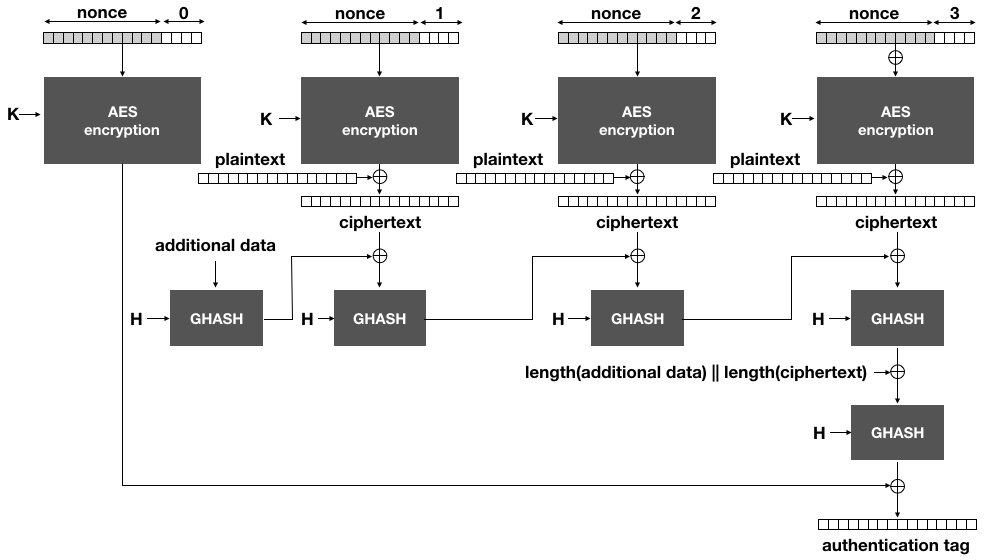
\includegraphics[width=0.8\linewidth]{gambar/aesgcm.png}
    \caption{Diagram alur AES-GCM}
    \label{fig:aesgcm}
\end{figure}

Dalam GCM, IV pada dasarnya adalah nonce yang harus unik dalam konteks penggunaan kunci tertentu. Keunikan nonce merupakan syarat penting karena kelemahan atau penggunaan ulang nonce dapat merusak jaminan keamanan GCM\cite{Chung2025Making}. Bukti yang lebih baru juga menunjukkan bahwa keamanan GCM dibatasi oleh jumlah blok dan kueri yang diproses, serta beberapa varian baru dikembangkan untuk memperbaiki batas keamanan tersebut\cite{Anh2026Refining}. Analisis lain bahkan melaporkan bahwa GCM dengan random IV 96-bit memberikan tingkat keamanan kurang dari 97 bit, sehingga konstruksi IV perlu dilakukan dengan hati-hati\cite{Mattsson2024Collision}.

Kombinasi AES dengan GCM menghasilkan skema AES-GCM, yang termasuk kategori AEAD karena menyediakan kerahasiaan sekaligus autentikasi dan integritas data\cite{Anh2026Refining}. Pada konfigurasi AES-256-GCM, AES-256 menyediakan enkripsi dengan kunci 256 bit dan 14 round, sedangkan GCM menyediakan pemrosesan IV, AAD, dan pembentukan tag autentikasi. Dengan demikian, penggunaan AES-256-GCM pada sistem berkas ruang pengguna sesuai untuk melindungi isi data sekaligus mendeteksi perubahan yang tidak sah terhadap data\cite{Anh2026Refining}.

\subsection{Argon2id}
Argon2id merupakan salah satu varian dari algoritma Argon2, yaitu fungsi hash kata sandi (password hashing function) yang keluar sebagai pemenang Password Hashing Competition pada tahun 2015\cite{}. Argon2 dirancang untuk menghasilkan turunan kunci (derived key) dari suatu masukan, umumnya berupa kata sandi, dengan tingkat ketahanan yang tinggi terhadap serangan brute-force maupun serangan menggunakan perangkat keras khusus seperti GPU, FPGA, dan ASIC\cite{}. Argon2 memiliki tiga varian utama, yaitu Argon2d, Argon2i, dan Argon2id. Argon2d mengakses memori dengan pola yang bergantung pada data (data-dependent), sehingga lebih tahan terhadap serangan trade-off waktu dan memori, namun rentan terhadap serangan side-channel. Argon2i mengakses memori dengan pola yang tidak bergantung pada data (data-independent), sehingga lebih tahan terhadap serangan side-channel namun memerlukan lebih banyak iterasi untuk mencapai tingkat keamanan yang setara. Argon2id merupakan kombinasi dari kedua pendekatan tersebut, yaitu menggunakan akses memori data-independent pada tahap awal proses dan data-dependent pada tahap selanjutnya, sehingga menghasilkan keseimbangan antara ketahanan terhadap serangan side-channel dan serangan trade-off waktu-memori\cite{}.

Argon2id tergolong sebagai fungsi hash yang memory-hard, yaitu fungsi yang dirancang agar proses komputasinya memerlukan alokasi memori dalam jumlah besar, bukan hanya waktu komputasi yang lama\cite{}. Karakteristik ini menjadikan Argon2id sulit dipercepat menggunakan perangkat keras paralel seperti GPU atau ASIC, karena perangkat tersebut umumnya unggul dalam komputasi paralel namun memiliki keterbatasan pada kapasitas memori berkecepatan tinggi yang dibutuhkan. Dengan demikian, upaya serangan brute-force terhadap kata sandi menggunakan perangkat keras khusus menjadi jauh lebih mahal secara sumber daya dibandingkan terhadap fungsi hash konvensional seperti SHA-256 atau bahkan fungsi hash kata sandi generasi sebelumnya seperti PBKDF2\cite{}.

Proses komputasi Argon2id dikendalikan oleh tiga parameter utama, yaitu memory cost (m), yang menentukan jumlah memori yang dialokasikan selama komputasi; time cost (t), yang menentukan jumlah iterasi atau pass yang dilakukan terhadap memori tersebut; dan parallelism (p), yang menentukan derajat paralelisme atau jumlah thread yang digunakan selama komputasi\cite{}. Ketiga parameter tersebut dapat disesuaikan untuk menyeimbangkan antara tingkat keamanan yang dihasilkan dengan sumber daya komputasi dan waktu eksekusi yang tersedia pada perangkat yang menjalankannya.

Dalam konteks penelitian ini, Argon2id digunakan sebagai mekanisme untuk menurunkan kunci kriptografis dari kata sandi yang dimasukkan oleh pengguna. Alih-alih menggunakan kata sandi secara langsung sebagai kunci enkripsi, kata sandi tersebut beserta suatu nilai acak yang disebut salt diproses melalui Argon2id untuk menghasilkan sebuah master key dengan panjang dan tingkat keacakan yang sesuai untuk digunakan pada algoritma AES-256-GCM. Penggunaan Argon2id pada tahap ini bertujuan untuk memperlambat upaya serangan brute-force terhadap kata sandi pengguna, mengingat kata sandi pada umumnya memiliki tingkat entropi yang jauh lebih rendah dibandingkan kunci kriptografis yang dihasilkan secara acak\cite{}.

\subsection{HKDF}
HMAC-based Extract-and-Expand Key Derivation Function (HKDF) merupakan fungsi turunan kunci (key derivation function) berbasis HMAC (Hash-based Message Authentication Code) yang distandarisasi melalui RFC 5869\cite{}. Berbeda dengan Argon2id yang dirancang untuk menurunkan kunci dari masukan dengan entropi rendah seperti kata sandi, HKDF dirancang untuk menurunkan satu atau lebih kunci kriptografis dari suatu bahan kunci awal (input keying material) yang sudah memiliki tingkat keacakan atau entropi yang cukup tinggi, seperti master key yang dihasilkan oleh Argon2id\cite{}.

Proses kerja HKDF terdiri atas dua tahap utama, yaitu tahap extract dan tahap expand\cite{}. Pada tahap extract, bahan kunci awal (input keying material) dikombinasikan dengan sebuah nilai salt menggunakan fungsi HMAC untuk menghasilkan sebuah pseudorandom key (PRK) dengan panjang tetap. Tahap ini bertujuan untuk memadatkan (condense) bahan kunci awal, yang mungkin memiliki distribusi keacakan yang tidak merata, menjadi sebuah kunci dengan tingkat keacakan yang seragam dan terstandarisasi\cite{}. Pada tahap expand, PRK yang dihasilkan dari tahap extract kemudian digunakan bersama sebuah parameter informasi konteks (info) untuk menghasilkan keluaran akhir (output keying material) dengan panjang yang dapat disesuaikan sesuai kebutuhan, melalui pemanggilan fungsi HMAC secara berulang terhadap PRK\cite{}.

Penggunaan parameter info pada tahap expand memungkinkan HKDF menghasilkan beberapa kunci turunan yang berbeda dari satu PRK yang sama, dengan cara memberikan nilai info yang berbeda untuk setiap tujuan penggunaan kunci\cite{}. Karakteristik ini menjadikan HKDF sesuai digunakan pada sistem yang memerlukan lebih dari satu kunci kriptografis dari satu sumber rahasia yang sama, misalnya kunci enkripsi data dan kunci untuk keperluan autentikasi, tanpa perlu menyimpan atau mengelola kunci-kunci tersebut secara terpisah.

Dalam konteks penelitian ini, HKDF digunakan pada tahap setelah proses turunan kunci menggunakan Argon2id. Master key yang dihasilkan oleh Argon2id dari kata sandi pengguna digunakan sebagai input keying material bagi HKDF, yang kemudian menurunkan kunci enkripsi spesifik yang digunakan oleh algoritma AES-256-GCM untuk setiap berkas atau setiap sesi penggunaan sistem. Pendekatan bertingkat ini, yaitu Argon2id untuk memperlambat serangan terhadap kata sandi dan HKDF untuk menurunkan kunci kerja dari master key, memungkinkan sistem berkas terenkripsi yang dibangun memiliki pemisahan yang jelas antara kunci induk dan kunci kerja, sehingga meningkatkan fleksibilitas dan keamanan pengelolaan kunci secara keseluruhan\cite{}.

\begin{table}[H]
    \centering
    \caption{Contoh tabel 1}
    \label{t-blok}
    \begin{tabular}{|c|l|l|}
        \hline
        \rowcolor[HTML]{C0C0C0}
        {\color[HTML]{000000} No.} & 
        \multicolumn{1}{c|}{\cellcolor[HTML]{C0C0C0}{\color[HTML]{000000} Nama}} & 
        \multicolumn{1}{c|}{\cellcolor[HTML]{C0C0C0}Fungsi} \\ 
        \hline
        
        \rowcolor[HTML]{FFFFFF}
        1 & \textit{Nama rincian objek yang akan dibahas 1} & Fungsi rincian objek penjelasan 1 \\ \hline
        2 & \textit{Nama rincian objek yang akan dibahas 2} & Fungsi rincian objek penjelasan 2 \\ \hline
        3 & \textit{Nama rincian objek yang akan dibahas 3} & Fungsi rincian objek penjelasan 3 \\ \hline
        4 & \textit{Nama rincian objek yang akan dibahas 4} & Fungsi rincian objek penjelasan 4 \\ \hline
    \end{tabular}
\end{table}


\subsection{Sub Dasar Teori III}
\lipsum[2]

\begin{figure}[H]
    \centering
    \includegraphics[width=0.8\linewidth]{gambar/diagram.png}
    \caption{Contoh gambar 1}
    \label{gambar1}
\end{figure}

\lipsum[2]


\section{Hipotesis}
\lipsum[2]

\begin{enumerate}
    \item \lipsum[2][4]
    \item \lipsum[2][4]
    \item \lipsum[2][4]
\end{enumerate}

\chapter[METODOLOGI PENELITIAN]{\\ METODELOGI PENELITIAN}

\section{Diagram Alir Metode Penelitian}
\lipsum[2]

\begin{figure}[H]
    \centering
    \includegraphics[width=0.40\linewidth]{gambar/flowchart.png}
    \caption{Contoh gambar 2}
    \label{gambar2}
\end{figure}

\section{Alat dan Bahan}

Pengerjaan proyek ini dilakukan dengan menggunakan perangkat keras dan perangkat lunak yang sesuai dengan kebutuhan dalam perancangan sistem. Perangkat-perangkat keras yang digunakan antara lain:

\begin{enumerate}
    \item Laptop \\ Pada pengerjaan proyek ini, laptop berfungsi sebagai perangkat utama dalam perancangan sistem sekaligus pengujian sistem. Laptop yang digunakan memiliki spesifikasi sebagaimana yang dimuat pada Tabel 3.1.
    \item SSD
\end{enumerate}

Adapun perangkat lunak yang digunakan pada proyek ini, berjalan pada perangkat keras yang digunakan dan berfungsi sebagai komponen utama dalam perancangan sistem. Perangkat-perangkat lunak yang digunakan meliputi:

\begin{enumerate}
    \item Linux Kernel 5.6+
    \item FUSE 3.10+ (API FUSE versi 35+)
    \item OpenSSL 3.0+
    \item libargon2
    \item C++20
    \item Neovim
    \item Git
    \item CMake 3.21+
    \item Perf 
    \item fio 
    \item hyperfine
\end{enumerate}

\section{Tahapan Penelitian}

Penelitian ini dilakukan secara sistematis dan terbagi dalam empat tahapan, diantaranya adalah perencanaan, perancangan sistem, pengujian sistem dan pengumpulan data, dan pengolahan data dan penyusunan laporan. Rincian tahapan penelitian ini dimuat dalam diagram alir (flowchart) pada gambar 3.2.

\begin{figure}[H]
    \centering
    \includegraphics[width=0.40\linewidth]{gambar/flowchart.png}
    \caption{Contoh gambar 3}
    \label{gambar3}
\end{figure}

Berdasarkan flowchart tahapan penelitian diatas, berikut uraian dari masing-masing tahapan:

\begin{enumerate}
    \item Perencanaan \\ Tahap pertama yang dilakukan dalam penelitian ini adalah perencanaan yang dimulai dari mengidentifikasi permasalahan yang menjadi latar belakang penelitian ini dilaksanakan. Kemudian dilakukan studi literatur untuk mengkaji dan mempelajari penelitian yang telah dilakukan beserta solusi yang telah diajukan. Hasil dari studi literatur menjadi dasar pertimbangan dalam perancangan sistem yang akan dilakukan dalam penelitian ini. Hasil dari tahapan ini berupa rumusan masalah, batasan masalah, hipotesis, serta rincian alat dan bahan yang akan digunakan dalam penelitian ini.
    \item Perancangan Sistem \\ Tahap perancangan sistem terdiri dari beberapa rincian tahapan yang diperlukan untuk memastikan sistem yang dibangun berjalan sebagaimana mestinya. Rincian tahapan yang dilakukan adalah sebagai berikut:
        \begin{enumerate}
            \item Perencanaan Arsitektur \\ Perencanaan bla bla bla
            \item Perencanaan Arsitektur \\ Perencanaan bla bla bla
        \end{enumerate}
    \item Pengujian Sistem dan Pengumpulan Data \\ \lipsum[3]
    \item Pengolahan Data dan Penyusunan Laporan \\ \lipsum[3]
\end{enumerate}

\section{Perancangan Sistem}
\subsection{Arsitektur Sistem}

Sistem terdiri dari tiga mode, yaitu:

\begin{enumerate}
    \item Inisialisasi \\ Pada mode ini, pengguna menenentukan direktori yang akan digunakan sistem berkas pengguna (FUSE) sekaligus menghasilkan file konfigurasi yang disimpan di dalam direktori tersebut.
    \item Mounting Filesystem \\ Mode utama yang digunakan setelah menentukan direktori yang digunakan dan file konfigurasi (.leichfs.conf) ditemukan.
    \item Pergantian Master Key \\ Mode ini digunakan untuk mengubah Master Key yang tersimpan dalam file konfigurasi.
\end{enumerate}

\subsection{Manajemen Kunci}

Sistem menggunakan tiga level kunci untuk bekerja. Ketiga kunci yang dimaksud adalah sebagai berikut

\begin{table}[H]
    \centering
    \caption{Daftar kunci yang digunakan pada sistem}
    \label{t:tabel-kunci-sistem}

    \begin{tabularx}{\textwidth}{|
        >{\centering\arraybackslash}p{1cm}|
        >{\arraybackslash}p{4cm}|
        >{\arraybackslash}X|}
        \hline

        \rowcolor[HTML]{C0C0C0}
        \textbf{Level}
        & \textbf{Kunci}
        & \textbf{Fungsi} \\
        \hline

        1
        & Wrapping Key (KEK)
        & Digunakan untuk membungkus (wrap) Master Key.
          KEK diturunkan melalui Argon2id dari passphrase
          dan salt yang tersimpan di
          \texttt{.leichfs.conf} pada setiap proses inisialisasi
          atau mount. Bersifat ephemeral dan dihapus (zeroization) setelah
          digunakan. \\
        \hline

        2
        & Master Key
        & Merupakan kunci utama yang digunakan sebagai dasar
          pembentukan File Key. Master Key dibangkitkan satu kali
          melalui \texttt{getrandom(2)} pada saat inisialisasi
          dan disimpan dalam keadaan terenkripsi (wrapped) menggunakan
          AES-256-GCM di \texttt{.leichfs.conf}. \\
        \hline

        3
        & File Key
        & Digunakan untuk mengenkripsi dan mendekripsi berkas.
          File Key diturunkan melalui HKDF-SHA256
          dari Master Key dengan \texttt{file\_salt} yang tersimpan
          pada file header. File Key dibuat untuk masing-masing berkas
          dan disimpan secara efemeral di \texttt{FH::file\_key}
          saat \texttt{open()} lalu dihapus (zeroization) saat
          \texttt{close()}. \\
        \hline

    \end{tabularx}
\end{table}

Kombinasi dari ketiga kunci tersebut membentuk pengamanan berkas melalui metode Envelope Encryption. Metode ini mengamankan data dengan menggunakan dua lapis kunci secara bersamaan 

\subsection{Format Penyimpanan Berkas}

Penyimpanan berkas pada sistem dilakukan dengan menambahkan header untuk masing-masing berkas yang terenkripsi. Setiap berkas juga dipecah menjadi sejumlah bagian yang disebut chunk dengan ukuran 65.536 byte. Seluruh chunk dari satu berkas diproses oleh sistem satu-persatu. Adapun detail struktur header adalah sebagai berikut:

\begin{table}[H]
    \centering
    \caption{Header yang digunakan pada sistem}
    \label{t:tabel-header-sistem}

    \begin{tabularx}{\textwidth}{|
        >{\centering\arraybackslash}p{1.5cm}|
        >{\centering\arraybackslash}p{2cm}|
        >{\centering\arraybackslash}p{3cm}|
        >{\centering\arraybackslash}p{2.5cm}|
        >{\arraybackslash}X|}
        \hline

        \rowcolor[HTML]{C0C0C0}
        \textbf{Offset}
        & \textbf{Size}
        & \textbf{Field}
        & \textbf{Type}
        & \textbf{Description} \\
        \hline

        0
        & 8 Bytes
        & \texttt{magic}
        & \texttt{uint8\_t[8]}
        & Identitas file dengan nilai \texttt{"LEICHFSX"}. \\
        \hline

        8
        & 4 Bytes
        & \texttt{version}
        & \texttt{uint32\_t}
        & Versi format file. Saat ini bernilai 1. \\
        \hline

        12
        & 4 Bytes
        & \texttt{chunk\_sz}
        & \texttt{uint32\_t}
        & Jumlah byte plaintext dalam setiap chunk. \\
        \hline

        16
        & 16 Bytes
        & \texttt{salt}
        & \texttt{uint8\_t[16]}
        & Salt acak per-file yang digunakan dalam proses HKDF. \\
        \hline

        32
        & 24 Bytes
        & \texttt{reserved}
        & \texttt{uint8\_t[24]}
        & Ruang yang dicadangkan untuk pengembangan format pada masa mendatang dan saat ini diisi dengan nilai nol. \\
        \hline

        56
        & 8 Bytes
        & \texttt{plain\_len\_be}
        & \texttt{uint64\_t}
        & Ukuran total plaintext dalam byte dalam representasi kanonis. \\
        \hline

    \end{tabularx}
\end{table}

Setiap chunk pada file diverifikasi melalui Additional Authentication Data (AAD). AAD merupakan kumpulan data unik yang digunakan untuk memverifikasi integritas data yang dienkripsi. Penggunaan AAD dalam kasus ini berperan untuk memverifikasi setiap chunk dari berkas. AAD yang digunakan tersusun dari data sepanjang 40 byte dengan rincian sebagai berikut:

\begin{itemize}
    \item magic
    \item version
    \item chunk\_sz
    \item salt
    \item chunk\_id
\end{itemize}

Dengan demikian, penggunaan AAD mengikat setiap chunk sesuai dengan urutannya pada berkas.

Adanya penambahan data pada berkas yang terenkripsi tentunya menimbulkan perbedaan ukuran berkas asli dengan berkas yang telah terenkripsi. Perbedaan ini dapat dihitung berdasarkan selisih antara ukuran data asli (plaintext) dan ukuran data setelah dienkripsi (ciphertext). 

\subsection{Alur Operasi Read-Write}
\lipsum[2]

\subsection{Manajemen Akses}
\lipsum[2]

\subsection{Modul Internal}
\lipsum[2]

\begin{table}[H]
    \centering
    \caption{Contoh tabel 2}
    \label{t-perbandinganRespon}
    \begin{tabular}{lllll}
        \hline
        \multirow{2}{*}{Karakteristik} & \multicolumn{4}{c}{Perbandingan performa} \\ 
        \cline{2-5}
        & \multicolumn{1}{c}{\textbf{PID}} 
        & \multicolumn{1}{c}{\textbf{MF3}} 
        & \multicolumn{1}{c}{\textbf{MF5}} 
        & \multicolumn{1}{c}{\textbf{MF7}} \\ 
        \hline
        
        \textit{Rise time} (s)     & 1,0580 & 1,0740 & 1,0620 & \textbf{1,0450} \\
        \textit{Settling time} (s) & 1,3380 & 1,3410 & 1,3350 & \textbf{1,3290} \\
        \textit{Overshoot} (\%)    & 0,0910 & 0,0440 & 0,0593 & \textbf{0,0121} \\
        \textit{Peak}              & 1,0910 & 1,0440 & 1,0593 & \textbf{1,0121} \\
        \textit{Peak time} (s)     & 1,0840 & 1,3560 & 1,2710 & 1,0520 \\ 
        \hline
    \end{tabular}
\end{table}

\lipsum[2]

\section{Pengambilan Data}
\lipsum[2]

\begin{table}[H]
    \centering
    \caption{Contoh tabel 3}
    \label{t-bestfits}
    \begin{tabular}{|
        >{\columncolor[HTML]{C0C0C0}}c|
        *{6}{>{\columncolor[HTML]{FFFFFF}}c|}}
        \hline
        
        \diagbox[
            width=5cm,
            height=1.5cm
        ]{\textit{Transfer Function}}{\textit{Validation Data}}
        & \cellcolor[HTML]{C0C0C0}\textbf{Data-1}
        & \cellcolor[HTML]{C0C0C0}\textbf{Data-2}
        & \cellcolor[HTML]{C0C0C0}\textbf{Data-3}
        & \cellcolor[HTML]{C0C0C0}\textbf{Data-4}
        & \cellcolor[HTML]{C0C0C0}\textbf{Data-5}
        & \cellcolor[HTML]{C0C0C0}\textbf{Data-6} \\
        \hline
        
        \cellcolor[HTML]{EFEFEF}$TF_{1}$ & 83,13 & 77,73 & 80,74 & 94,22 & 85,88 & 83,76 \\ \hline
        \cellcolor[HTML]{EFEFEF}$TF_{2}$ & 79,61 & 83,34 & 76,93 & 84,30 & 82,39 & 77,31 \\ \hline
        \cellcolor[HTML]{EFEFEF}$TF_{3}$ & 81,88 & 72,91 & 82,17 & 95,17 & 84,90 & 81,90 \\ \hline
        \cellcolor[HTML]{EFEFEF}$TF_{4}$ & 82,60 & 73,58 & 81,63 & 96,21 & 85,44 & 84,23 \\ \hline
        \cellcolor[HTML]{EFEFEF}$TF_{5}$ & 83,13 & 77,33 & 80,95 & 94,59 & 85,89 & 83,87 \\ \hline
        \cellcolor[HTML]{EFEFEF}$TF_{6}$ & 83,56 & 73,29 & 81,42 & 96,17 & 85,40 & 84,33 \\ \hline
    \end{tabular}
\end{table}

\lipsum[2]


\chapter[RENCANA DAN JADWAL KEGIATAN]{\\ RENCANA DAN JADWAL KEGIATAN}

\section{Jadwal Kerja PA}
\lipsum[2][4]

\begin{table}[h!]
    \centering
    \caption{Tabel Rencana Kegiatan (contoh)}
    \label{t-rencana-kegiatan}
    \begin{tabular}{|c|p{2.5cm}|c|c|c|c|c|c|p{3.5cm}|}
        \hline
        \multirow{2}{*}{\textbf{No}} 
        & \multirow{2}{*}{\textbf{Kegiatan}} 
        & \multicolumn{6}{c|}{\textbf{Bulan}} 
        & \multirow{2}{*}{\textbf{Target capaian}} \\ 
        \cline{3-8}
        
        & & \textbf{Des} & \textbf{Jan} & \textbf{Feb} & \textbf{Mar} & \textbf{Apr} & \textbf{Mei} & \\ 
        \hline
        
        1 & Studi Literatur 
            & \cellcolor[HTML]{C0C0C0} & \cellcolor[HTML]{C0C0C0} & \cellcolor[HTML]{C0C0C0} 
            & & & & Pengetahuan tentang penelitian sebelumnya dan memahami RL dan MADDPG \\ \hline
            
        2 & Perancangan awal sistem 
            & & \cellcolor[HTML]{C0C0C0} & \cellcolor[HTML]{C0C0C0} 
            & & & & Merancang garis besar dengan mencari referensi sumber terbuka \\ \hline
            
        3 & Pengerjaan sistem 
            & & & \cellcolor[HTML]{C0C0C0} & \cellcolor[HTML]{C0C0C0} 
            & & & Pengerjaan simulasi dan sistem MADDPG \\ \hline
            
        4 & Pengujian sistem 
            & & & & \cellcolor[HTML]{C0C0C0} & \cellcolor[HTML]{C0C0C0} 
            & & Pengujian simulasi dan sistem MADDPG \\ \hline
            
        5 & Pengambilan data 
            & & & & \cellcolor[HTML]{C0C0C0} & \cellcolor[HTML]{C0C0C0} 
            & & Pengambilan data latih dan data testing \\ \hline
            
        6 & Pengerjaan sistem 
            & & & & & \cellcolor[HTML]{C0C0C0} & \cellcolor[HTML]{C0C0C0} 
            & Pembuatan laporan \\ \hline
    \end{tabular}
\end{table}

\input{chapters/daftarpustaka}
\input{chapters/lampiran}

% Catatan pribadi
\input{Note.tex}
\end{document}

